\documentclass[a4paper]{article}

\usepackage[left=2cm,right=2cm,top=2cm,bottom=1.5cm]{geometry}

% General style
\usepackage{newunicodechar}
\newunicodechar{→}{\fontspec{Gentium Plus}→}
\newunicodechar{–}{--}
\newunicodechar{“}{``}
\newunicodechar{”}{''}
\newunicodechar{‘}{`}
\newunicodechar{’}{'}

% Formulas
\usepackage{amsmath}
\usepackage{amssymb}

% Internal references
\usepackage{hyperref}
\usepackage[capitalize]{cleveref}

% Figures
\usepackage{subcaption}
\usepackage[font=small,labelfont=it]{caption}
\usepackage{graphicx}
\usepackage{tikz}
\usetikzlibrary{arrows}
\usetikzlibrary{arrows.meta}
\usetikzlibrary{decorations.pathreplacing}
\usetikzlibrary{bayesnet}
\usepackage[linguistics,edges]{forest}
\usepackage{rotating}

% Bibliography
\usepackage[backend=biber,
            bibstyle=numeric-comp, %biblatex-sp-unified,
            citestyle=numeric-comp,
            sorting=none,
            maxcitenames=2,url=false,
            maxbibnames=10]{biblatex}
\addbibresource{library.bib}
\def\bibfont{\fontfamily{\rmdefault}\fontseries{m}\fontshape{n}\fontsize{9}{11}\selectfont}

\renewbibmacro*{doi+eprint+url}{%
  \printfield{doi}%
  \newunit\newblock%
  \iftoggle{bbx:eprint}{%
    \usebibmacro{eprint}%
  }{}%
  \newunit\newblock%
  \iffieldundef{doi}{%
    \usebibmacro{url+urldate}}%
  {}%
}

\newcommand{\glot}[2]{#1 {\scriptsize{[\texttt{\href{https://glottolog.org/resource/languoid/id/#2}{#2}}]}}}

% Code inclusion with syntax highlighting
\usepackage{minted}
\setminted{fontsize=\tiny,baselinestretch=0.9}



\title{Supplementary material: Clocks with bursts: Phylogenetic inference of schismogenesis in language evolution}
\date{}
\author{
  Gereon A. Kaiping$^{1}$,
  Nico Neureiter$^{1}$\\[2ex]
  $^{1}$Geographic Information Science Center, Universität Zürich, CH
}

\begin{document}
\maketitle
\renewcommand{\thepage}{S\arabic{page}} 
\renewcommand{\thesection}{S\arabic{section}}  
\renewcommand{\thetable}{S\arabic{table}}  
\renewcommand{\thefigure}{S\arabic{figure}}
\renewcommand{\figurename}{Figure} 

\section{Tree heights}
We have reconstructed phylogenetic trees for the Austronesian, Bantu, Indo-European and Sino-Tibetan language families using different clock models. Figure~\ref{fig:tree_height} shows the reconstructed tree height for each of these families according to strict and relaxed clock with and without bursts.

\begin{figure}[h]
  \centering
  \begin{subfigure}{0.4\textwidth}
    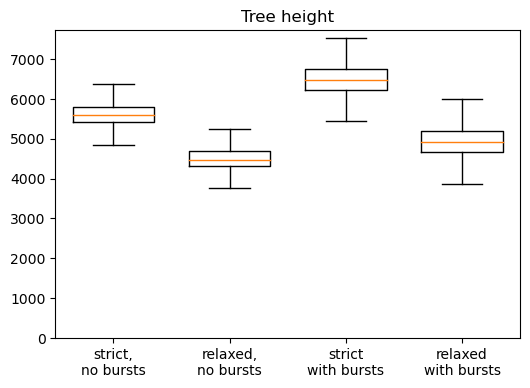
\includegraphics[width=\textwidth]{supplement/analysis/austronesian_treeheight.png}
    \caption{Austronesian}
    \label{fig:tree_height:austronesian}
  \end{subfigure}
  \begin{subfigure}{0.4\textwidth}
    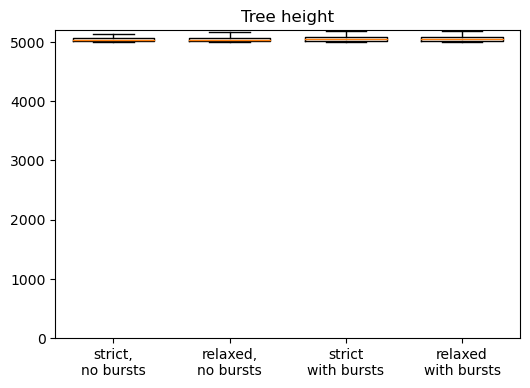
\includegraphics[width=\textwidth]{supplement/analysis/bantu_treeheight.png}
    \caption{Bantu language}
    \label{fig:tree_height:bantu}
  \end{subfigure}

  \begin{subfigure}{0.4\textwidth}
    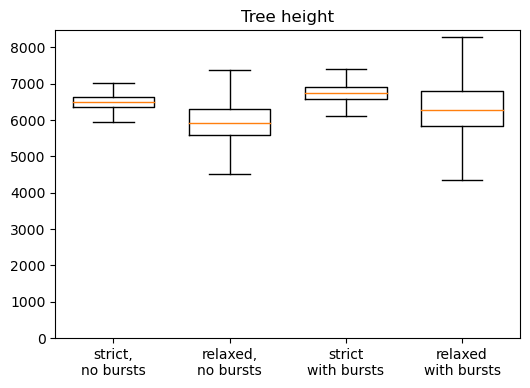
\includegraphics[width=\textwidth]{supplement/analysis/indoeuropean_treeheight.png}
    \caption{Indo-European}
    \label{fig:tree_height:indoeuropean}
  \end{subfigure}
  \begin{subfigure}{0.4\textwidth}
    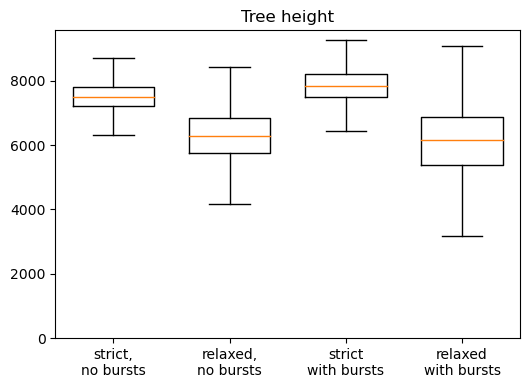
\includegraphics[width=\textwidth]{supplement/analysis/sinotibetan_treeheight.png}
    \caption{Sino-Tibetan}
    \label{fig:tree_height:sinotibetan}
  \end{subfigure}
  
  \caption{The tree height, i.\,e. the age of the most recent common ancestor of all leaves, for the Austronesian, Bantu, Indo-European and Sino-Tibetan language families according to different clock models.}
  \label{fig:tree_height}
\end{figure}


\newpage
\section{Branch rate variation}

\begin{figure}[h]
  \centering
  \begin{subfigure}{0.4\textwidth}
    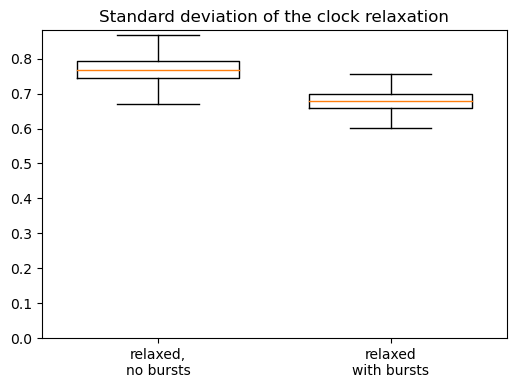
\includegraphics[width=\textwidth]{supplement/analysis/austronesian_clockrates.png}
    \caption{Austronesian}
    \label{fig:rate_variation:austronesian}
  \end{subfigure}
  \begin{subfigure}{0.4\textwidth}
    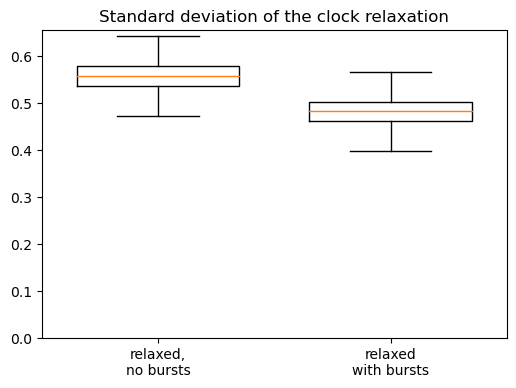
\includegraphics[width=\textwidth]{supplement/analysis/bantu_clockrates.png}
    \caption{Bantu}
    \label{fig:rate_variation:bantu}
  \end{subfigure}
  \begin{subfigure}{0.4\textwidth}
    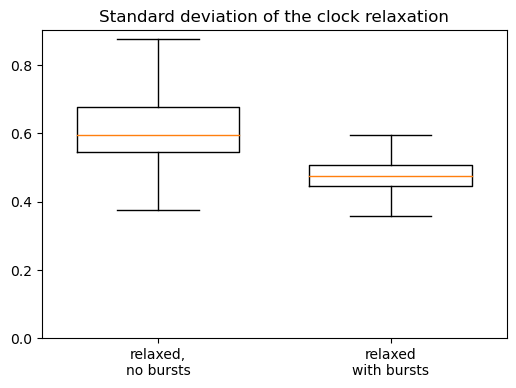
\includegraphics[width=\textwidth]{supplement/analysis/indoeuropean_clockrates.png}
    \caption{Indo-European}
    \label{fig:rate_variation:indoeuropean}
  \end{subfigure}
  \begin{subfigure}{0.4\textwidth}
    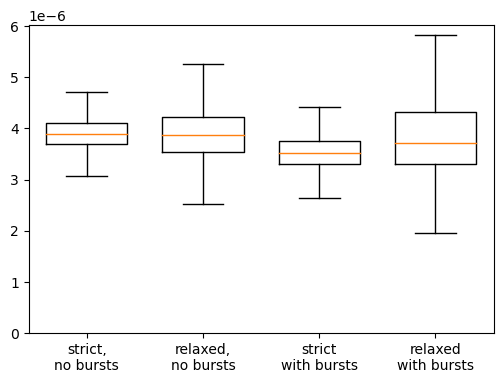
\includegraphics[width=\textwidth]{supplement/analysis/sinotibetan_clockrates.png}
    \caption{Sino-Tibetan}
    \label{fig:rate_variation:sinotibetan}
  \end{subfigure}
  
  \caption{The branch rate variation in the four language families for the relaxed clock with and without bursts.}
  \label{fig:rate_variation}
\end{figure}

\newpage
\section{Beast2 configuration files and run results}
The supplementary data repository at \url{http://doi.org/10.17605/OSF.IO/8M3RJ}
contains the following additional file collections.
\begin{description}
\item[\texttt{supplement.pdf}] This document.
\item[\texttt{beast.zip}] The burst clock extension for Beast2 used in the paper.
\item[\texttt{supplement.zip}] The code to generate the configuration files and analyse
  all runs. This means
  \begin{enumerate}
  \item the Python code to download a well-specified
    version of the data repository for each of the four language families,
  \item the template Beast2 XML file embedded as code fragments into a literate
    programming Markdown file,
  \item for each language family a Makefile recipe to
    generate all Beast2 configuration file from the template,
  \item the Python scripts containing the individual transformations used in
    (3),
  \item the Python script used to analyse the MCMC runs (see below for the raw MCMC output) and
  \item the figures generated by that analysis (also contained in the
    article or in this document)
  \end{enumerate}
\item[\texttt{austronesian.zip}] The complete result set (including the
  sampled trees and raw log files, and the screen log used to estimate run
  times) for all 22 Austronesian runs.
\item[\texttt{bantu.zip}] The complete result set (including the
  sampled trees and raw log files, and the screen log used to estimate run
  times) for all 20 Bantu runs.
\item[\texttt{indoeuropean.zip}] The complete result set (including the
  sampled trees and raw log files, and the screen log used to estimate run
  times) for all 20 Indo-European runs.
\item[\texttt{sinotibetan.zip}] The complete result set (including the
  sampled trees and raw log files, and the screen log used to estimate run
  times) for all 20 Sino-Tibetan runs.
\end{description}
\end{document}